\section{Design}

\subsection{System Architecture Diagrams}

\subsubsection{Component-Level Architecture}

The dual-sensor temperature monitoring system connects seven hardware components to the Arduino Mega 2560 microcontroller through four distinct interfaces: ADC (analog), OneWire (digital), I2C (LCD), and GPIO (LEDs). The component-level architecture diagram in \citeimg{fig:system_structural_diagram} illustrates the physical topology and communication protocols between all system elements.

The NTC thermistor connects through a voltage divider to analog pin A0, providing a continuously variable voltage that the ADC samples at each acquisition cycle. The DS18B20 connects through a single OneWire data line (with a 4.7 k$\Omega$ pull-up resistor) to digital pin 2, communicating temperature readings as digital data packets. The LCD 1602 connects via the I2C bus (SDA on pin 20, SCL on pin 21), allowing the display to be updated with formatted temperature and status information. Three LEDs connect through current-limiting resistors to digital pins 8, 9, and 10, providing immediate visual feedback on system status and alert conditions.

\begin{figure}[H]
\centering
\begin{tikzpicture}[
    comp/.style={draw, rectangle, rounded corners, minimum width=3.5cm,
                 minimum height=1.0cm, text centered, align=center, fill=blue!10},
    mcu/.style={draw, rectangle, rounded corners, minimum width=4.0cm,
                minimum height=1.2cm, text centered, align=center, fill=green!15, line width=1.2pt},
    conn/.style={->, thick, >=Stealth}]

    % MCU at center
    \node[mcu] (mcu) at (0, 0) {Arduino Mega 2560\\ATmega2560};

    % Sensors on the left
    \node[comp, fill=red!10] (ntc) at (-6.5, 2.0) {NTC Thermistor\\10K, $\beta$=3950};
    \node[comp, fill=red!10] (ds)  at (-6.5, -2.0) {DS18B20\\Digital Temp};

    % Display on the right top
    \node[comp, fill=yellow!15] (lcd) at (6.5, 2.0) {LCD 1602\\I2C Display};

    % LEDs on the right bottom
    \node[comp, fill=green!15] (ledg) at (5.0, -1.5) {Green LED\\(Normal)};
    \node[comp, fill=red!15]   (ledr) at (5.0, -2.8) {Red LED\\(Analog Alert)};
    \node[comp, fill=orange!15](ledy) at (5.0, -4.1) {Yellow LED\\(Digital Alert)};

    % Serial out bottom
    \node[comp, fill=gray!15] (uart) at (0, -4.5) {Serial Terminal\\(STDIO via UART)};

    % Connections
    \draw[conn, orange] (ntc.east) -- node[above, font=\scriptsize]{ADC (A0)} (mcu.west |- ntc);
    \draw[conn, blue]   (ds.east)  -- node[below, font=\scriptsize]{OneWire (D2)} (mcu.west |- ds);
    \draw[conn, green!60!black] (mcu.east |- lcd) -- node[above, font=\scriptsize]{I2C (SDA/SCL)} (lcd.west);
    \draw[conn] (mcu.east |- ledg) -- node[above, font=\scriptsize]{GPIO D8} (ledg.west);
    \draw[conn] (mcu.east |- ledr) -- node[above, font=\scriptsize]{GPIO D9} (ledr.west);
    \draw[conn] (mcu.east |- ledy) -- node[above, font=\scriptsize]{GPIO D10} (ledy.west);
    \draw[conn, <->] (mcu.south) -- node[right, font=\scriptsize]{UART 9600} (uart.north);
\end{tikzpicture}
\caption{System structural diagram --- component-level architecture}
\label{fig:system_structural_diagram}
\end{figure}

The data flows in the system follow distinct paths. Sensor data flows inward from the NTC thermistor and DS18B20 into the microcontroller, where it is processed by the acquisition and conditioning pipeline. Processed results flow outward through two channels: the I2C bus to the LCD for real-time display, and the UART serial port for detailed STDIO reports. Control signals flow outward through GPIO to the LEDs for immediate visual status indication.

\subsubsection{Layered System Architecture}

The software architecture follows a layered design pattern that separates hardware-specific drivers from application logic, enabling code reuse across laboratory projects and simplifying maintenance. \citeimg{fig:layered_architecture} illustrates the five-layer hierarchy used in this system.

\begin{figure}[H]
\centering
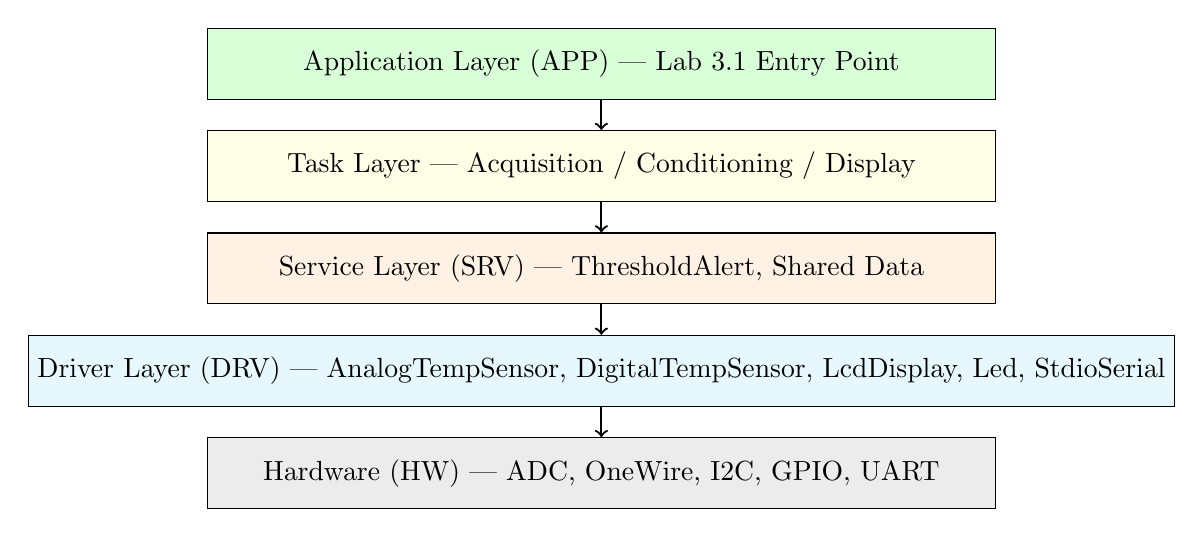
\begin{tikzpicture}[
    box/.style={draw, rectangle, minimum width=10cm, minimum height=0.9cm,
                text centered, align=center, fill=blue!10},
    node distance=0.4cm]
    \node[box, fill=green!15]  (app)  at (0, 0)    {Application Layer (APP) --- Lab 3.1 Entry Point};
    \node[box, fill=yellow!10] (task) at (0, -1.3)  {Task Layer --- Acquisition / Conditioning / Display};
    \node[box, fill=orange!10] (srv)  at (0, -2.6)  {Service Layer (SRV) --- ThresholdAlert, Shared Data};
    \node[box, fill=cyan!10]   (drv)  at (0, -3.9)  {Driver Layer (DRV) --- AnalogTempSensor, DigitalTempSensor, LcdDisplay, Led, StdioSerial};
    \node[box, fill=gray!15]   (hw)   at (0, -5.2)  {Hardware (HW) --- ADC, OneWire, I2C, GPIO, UART};
    \foreach \a/\b in {app/task, task/srv, srv/drv, drv/hw}
        \draw[->, thick] (\a) -- (\b);
\end{tikzpicture}
\caption{Layered software architecture of the dual-sensor monitoring system}
\label{fig:layered_architecture}
\end{figure}

The Hardware Layer (HW) encompasses the physical peripherals: the ADC for the NTC thermistor, the OneWire bus for the DS18B20, the I2C bus for the LCD, GPIO pins for the LEDs, and the UART for serial communication. The Driver Layer (DRV) contains reusable library modules that abstract hardware access behind clean C++ interfaces. The Service Layer (SRV) provides application-independent processing logic, including the ThresholdAlert module for hysteresis detection and the shared data structures with their synchronization primitives. The Task Layer defines the three FreeRTOS tasks that implement the monitoring pipeline. The Application Layer (APP) is the lab entry point that initializes hardware, creates synchronization primitives, spawns tasks, and starts the FreeRTOS scheduler.

Each layer communicates only with its immediate neighbor, ensuring that application code never directly manipulates hardware registers, and driver modules can be tested and reused independently of the specific application logic.

\subsubsection{FreeRTOS Task Architecture}

The three FreeRTOS tasks operate as a pipeline, with well-defined data flows and synchronization points. \citeimg{fig:task_architecture} shows the task communication topology.

\begin{figure}[H]
\centering
\begin{tikzpicture}[
    task/.style={draw, rectangle, rounded corners, minimum width=3.8cm,
                 minimum height=1.5cm, text centered, align=center, fill=blue!10, line width=1pt},
    data/.style={draw, rectangle, minimum width=2.5cm, minimum height=0.8cm,
                 text centered, align=center, fill=yellow!15, font=\small},
    sync/.style={draw, ellipse, minimum width=2.0cm, minimum height=0.7cm,
                 text centered, align=center, fill=orange!15, font=\small},
    arr/.style={->, thick, >=Stealth}]

    % Tasks
    \node[task] (t1) at (0, 0)    {Task 1\\\textbf{Acquisition}\\50 ms, Prio 3};
    \node[task] (t2) at (6, 0)    {Task 2\\\textbf{Conditioning}\\Event, Prio 2};
    \node[task] (t3) at (12, 0)   {Task 3\\\textbf{Display}\\500 ms, Prio 1};

    % Shared data
    \node[data] (sd) at (3, -2.5) {g\_sensorData};
    \node[data] (ad) at (9, -2.5) {g\_alertData};

    % Sync primitives
    \node[sync] (sem) at (3, 1.8) {Semaphore};
    \node[sync] (mtx) at (6, -4.0) {Mutex};

    % Arrows
    \draw[arr, blue] (t1) -- node[above, font=\scriptsize]{give} (sem);
    \draw[arr, blue] (sem) -- node[above, font=\scriptsize]{take} (t2);
    \draw[arr, red]  (t1.south) -- node[left, font=\scriptsize]{write} (sd.north west);
    \draw[arr, red]  (sd.north east) -- node[right, font=\scriptsize]{read} (t2.south);
    \draw[arr, red]  (t2.south) -- node[left, font=\scriptsize]{write} (ad.north west);
    \draw[arr, red]  (ad.north east) -- node[right, font=\scriptsize]{read} (t3.south);
    \draw[arr, dashed] (mtx) -- (sd);
    \draw[arr, dashed] (mtx) -- (ad);
\end{tikzpicture}
\caption{FreeRTOS task communication architecture}
\label{fig:task_architecture}
\end{figure}

Task 1 (Acquisition) runs at the highest priority (3) with a 50 ms period using \texttt{vTaskDelayUntil()} for drift-free timing. It reads both sensors, writes the results to \texttt{g\_sensorData} under mutex protection, and gives the binary semaphore to notify Task 2. Task 2 (Conditioning) runs at medium priority (2) and blocks on the semaphore until new data is available, then reads the sensor data, applies the threshold detection logic for both sensors, writes the alert status to \texttt{g\_alertData} under mutex protection, and updates the LED indicators. Task 3 (Display) runs at the lowest priority (1) with a 500 ms period, reading both shared data structures under mutex protection and formatting the output for the LCD and STDIO.

\subsection{Block Diagrams}

\subsubsection{Main Application Flowchart}

\citeimg{fig:app_flowchart} shows the overall initialization sequence performed by the \texttt{lab3\_1Setup()} function. After initialization completes, the FreeRTOS scheduler takes over and the three tasks run concurrently.

\tikzset{
    startstop/.style={rectangle, rounded corners, minimum width=3.0cm,
        minimum height=0.7cm, text centered, align=center, draw=black, fill=gray!15},
    process/.style={rectangle, minimum width=3.0cm,
        minimum height=0.7cm, text centered, align=center, draw=black, fill=blue!10},
    decision/.style={diamond, aspect=2.5, minimum width=2cm,
        minimum height=0.7cm, text centered, align=center, draw=black, fill=orange!15},
    io/.style={trapezium, trapezium left angle=70, trapezium right angle=110,
        minimum width=2.5cm, minimum height=0.7cm, text centered, align=center,
        draw=black, fill=green!10},
    arrow/.style={thick,->,>=Stealth}
}

\begin{figure}[H]
\centering
\begin{tikzpicture}
    \node (start)  [startstop] at (0,   0.0)   {Start};
    \node (stdio)  [process]   at (0,  -1.8)   {Initialize STDIO\\Serial (9600 baud)};
    \node (banner) [io]        at (0,  -3.8)   {Print startup\\banner to STDIO};
    \node (sync)   [process]   at (0,  -5.8)   {Create mutex and\\binary semaphore};
    \node (t1)     [process]   at (0,  -7.6)   {Create Task 1:\\Acquisition (Prio 3)};
    \node (t2)     [process]   at (0,  -9.4)   {Create Task 2:\\Conditioning (Prio 2)};
    \node (t3)     [process]   at (0, -11.2)   {Create Task 3:\\Display (Prio 1)};
    \node (sched)  [startstop] at (0, -13.0)   {FreeRTOS Scheduler\\starts automatically};

    \draw [arrow] (start)  -- (stdio);
    \draw [arrow] (stdio)  -- (banner);
    \draw [arrow] (banner) -- (sync);
    \draw [arrow] (sync)   -- (t1);
    \draw [arrow] (t1)     -- (t2);
    \draw [arrow] (t2)     -- (t3);
    \draw [arrow] (t3)     -- (sched);
\end{tikzpicture}
\caption{Main application initialization flowchart (\texttt{lab3\_1Setup})}
\label{fig:app_flowchart}
\end{figure}

\subsubsection{Sensor Acquisition Task Flowchart}

The acquisition task (\citeimg{fig:flowchart_acquisition}) implements the periodic reading of both temperature sensors. It uses a non-blocking approach for the DS18B20: on each cycle, it reads the result of the previous conversion and starts a new one, overlapping the conversion time with the next sleep period.

\begin{figure}[H]
\centering
\begin{tikzpicture}
    \node (start) [startstop] at (0,    0.0)  {Task Start};
    \node (init)  [process]   at (0,   -1.8)  {Initialize NTC\\and DS18B20 sensors};
    \node (req1)  [process]   at (0,   -3.6)  {Request first\\DS18B20 conversion};
    \node (wait)  [process]   at (0,   -5.6)  {vTaskDelayUntil\\(50 ms period)};
    \node (adc)   [process]   at (0,   -7.4)  {Read NTC via ADC\\Convert to \textdegree C};
    \node (dchk)  [decision]  at (0,  -10.0)  {DS18B20\\conversion\\complete?};
    \node (dread) [process]   at (5.5, -10.0)  {Read DS18B20\\temperature};
    \node (dlast) [process]   at (-5.5,-10.0)  {Use last known\\temperature};
    \node (dreq)  [process]   at (0,  -12.5)  {Request next\\DS18B20 conversion};
    \node (mtx)   [process]   at (0,  -14.3)  {Mutex: write to\\g\_sensorData};
    \node (sem)   [process]   at (0,  -16.1)  {Give semaphore\\to Task 2};

    \draw [arrow] (start) -- (init);
    \draw [arrow] (init)  -- (req1);
    \draw [arrow] (req1)  -- (wait);
    \draw [arrow] (wait)  -- (adc);
    \draw [arrow] (adc)   -- (dchk);
    \draw [arrow] (dchk)  -- node[above, font=\scriptsize]{Yes} (dread);
    \draw [arrow] (dchk)  -- node[above, font=\scriptsize]{No}  (dlast);
    \draw [arrow] (dread.south) -- (5.5, -12.5) -- (dreq);
    \draw [arrow] (dlast.south) -- (-5.5, -12.5) -- (dreq);
    \draw [arrow] (dreq)  -- (mtx);
    \draw [arrow] (mtx)   -- (sem);
    \draw [arrow] (sem.west) -- ++(-3.0, 0) |- (wait.west);
\end{tikzpicture}
\caption{Sensor acquisition task flowchart (Task 1)}
\label{fig:flowchart_acquisition}
\end{figure}

The NTC reading is fast (a single \texttt{analogRead()} call takes approximately 104 $\mu$s), while the DS18B20 conversion runs asynchronously. By starting the conversion at the end of each cycle and reading the result at the beginning of the next, the conversion time is hidden behind the 50 ms sleep period, maintaining consistent timing.

\subsubsection{Signal Conditioning Task Flowchart}

The conditioning task (\citeimg{fig:flowchart_conditioning}) is event-driven, waking only when the acquisition task signals new data via the binary semaphore. This approach eliminates polling overhead and ensures that conditioning always processes the most recent sensor data.

\begin{figure}[H]
\centering
\begin{tikzpicture}
    \node (start) [startstop] at (0,    0.0)  {Task Start};
    \node (init)  [process]   at (0,   -1.8)  {Initialize alerts\\and LEDs};
    \node (sem)   [process]   at (0,   -3.8)  {Take semaphore\\(block until given)};
    \node (read)  [process]   at (0,   -5.6)  {Mutex: read\\g\_sensorData};
    \node (aupd)  [process]   at (0,   -7.4)  {Update analog\\ThresholdAlert FSM};
    \node (dupd)  [process]   at (0,   -9.2)  {Update digital\\ThresholdAlert FSM};
    \node (write) [process]   at (0,  -11.0)  {Mutex: write\\g\_alertData};
    \node (led)   [process]   at (0,  -12.8)  {Update LEDs based\\on alert states};

    \draw [arrow] (start) -- (init);
    \draw [arrow] (init)  -- (sem);
    \draw [arrow] (sem)   -- (read);
    \draw [arrow] (read)  -- (aupd);
    \draw [arrow] (aupd)  -- (dupd);
    \draw [arrow] (dupd)  -- (write);
    \draw [arrow] (write) -- (led);
    \draw [arrow] (led.west) -- ++(-2.5, 0) |- (sem.west);
\end{tikzpicture}
\caption{Signal conditioning and alerting task flowchart (Task 2)}
\label{fig:flowchart_conditioning}
\end{figure}

\subsubsection{Threshold Alert FSM State Diagram}

The ThresholdAlert module implements a 4-state finite state machine (FSM) that governs the transition between normal and alert conditions. \citeimg{fig:fsm_threshold} shows the state diagram with transition conditions.

\begin{figure}[H]
\centering
\begin{tikzpicture}[>=Stealth, auto, node distance=4.5cm,
        every state/.style={draw, circle, minimum size=1.8cm, font=\small, align=center}]
    \node[state, initial]  (norm)  {NORMAL};
    \node[state]           (dbh)   [right of=norm]  {DEBOUNCE\\HIGH};
    \node[state]           (alert) [below of=dbh]   {ALERT\\ACTIVE};
    \node[state]           (dbl)   [left of=alert]  {DEBOUNCE\\LOW};

    \path[->]
        (norm)  edge              node[above] {$T > T_{high}$}       (dbh)
        (dbh)   edge [bend left]  node[right] {$N$ confirmations}    (alert)
        (dbh)   edge [bend right] node[above] {$T \leq T_{high}$}   (norm)
        (alert) edge              node[below] {$T < T_{low}$}       (dbl)
        (dbl)   edge [bend left]  node[left]  {$N$ confirmations}   (norm)
        (dbl)   edge [bend right] node[below] {$T \geq T_{low}$}   (alert);
\end{tikzpicture}
\caption{Threshold alert FSM state diagram with hysteresis and debounce}
\label{fig:fsm_threshold}
\end{figure}

In the NORMAL state, the system monitors the input value and transitions to DEBOUNCE\_HIGH when the value exceeds the high threshold ($T_{high}$ = 30\textdegree C). The DEBOUNCE\_HIGH state counts consecutive readings above the threshold; after $N$ confirmations (default 5), the system commits to the ALERT\_ACTIVE state. If the value drops back below the threshold before $N$ confirmations, the transition is cancelled and the system returns to NORMAL. Symmetrically, from ALERT\_ACTIVE, the system transitions to DEBOUNCE\_LOW when the value drops below the low threshold ($T_{low}$ = 28\textdegree C), and returns to NORMAL after $N$ confirmed readings below the threshold. This dual-layer protection ensures that both transient noise (filtered by debounce) and sustained oscillation near a single threshold (filtered by hysteresis) are handled robustly.

\subsubsection{Display Task Flowchart}

The display task (\citeimg{fig:flowchart_display}) runs periodically at 500 ms intervals, reading the latest sensor data and alert status to update both the LCD display and the serial terminal output. The LCD alternates between two information pages, and the STDIO report is generated every 4th cycle (2 seconds).

\begin{figure}[H]
\centering
\begin{tikzpicture}
    \node (start) [startstop] at (0,    0.0)  {Task Start};
    \node (init)  [process]   at (0,   -1.8)  {Initialize LCD\\Show startup message};
    \node (wait)  [process]   at (0,   -3.8)  {vTaskDelayUntil\\(500 ms period)};
    \node (read)  [process]   at (0,   -5.6)  {Mutex: read sensor\\and alert data};
    \node (page)  [decision]  at (0,   -8.1)  {LCD page\\number?};
    \node (p0)    [process]   at (-5.0,-8.1)  {Page 0: show\\temps + status};
    \node (p1)    [process]   at (5.0, -8.1)  {Page 1: show\\threshold config};
    \node (lcd)   [process]   at (0,  -10.5)  {Update LCD\\display lines};
    \node (rpt)   [decision]  at (0,  -13.0)  {Report\\cycle?};
    \node (print) [io]        at (5.0,-13.0)  {Print structured\\STDIO report};
    \node (skip)  [process]   at (-4.0,-13.0) {Skip report};

    \draw [arrow] (start) -- (init);
    \draw [arrow] (init)  -- (wait);
    \draw [arrow] (wait)  -- (read);
    \draw [arrow] (read)  -- (page);
    \draw [arrow] (page)  -- node[above, font=\scriptsize]{0} (p0);
    \draw [arrow] (page)  -- node[above, font=\scriptsize]{1} (p1);
    \draw [arrow] (p0.south)  -- (-5.0, -10.5) -- (lcd);
    \draw [arrow] (p1.south)  -- (5.0, -10.5) -- (lcd);
    \draw [arrow] (lcd)   -- (rpt);
    \draw [arrow] (rpt)   -- node[above, font=\scriptsize]{Yes} (print);
    \draw [arrow] (rpt)   -- node[above, font=\scriptsize]{No}  (skip);
    \draw [arrow] (print.east) -- ++(1.5, 0) |- (wait.east);
    \draw [arrow] (skip.west) -- ++(-1.5, 0) |- (wait.west);
\end{tikzpicture}
\caption{Display and reporting task flowchart (Task 3)}
\label{fig:flowchart_display}
\end{figure}

\subsection{Electrical Schematics}

The complete circuit schematic (\citeimg{fig:circuit_schematic}) shows all electrical connections between the Arduino Mega 2560 and peripheral components.

\begin{figure}[H]
\centering
\begin{circuitikz}[scale=0.85, transform shape]
    % Title area
    \node[font=\bfseries] at (5, 1.5) {Arduino Mega 2560 --- Dual Sensor Temperature Monitor};

    % NTC Thermistor voltage divider
    \draw (0, 0) node[anchor=east, font=\small]{5V}
        to[R, l=$10\,\mathrm{k}\Omega$, a=Series] (3, 0)
        to[short] (4.5, 0)
        node[anchor=west, font=\small]{A0};
    \draw (3, 0) to[short] (3, -1.5)
        to[thR, l_=NTC, a=10k] (3, -3.5)
        node[ground]{};
    \node[font=\scriptsize, anchor=west] at (4.5, -0.5) {(Analog Input)};

    % DS18B20
    \draw (0, -5) node[anchor=east, font=\small]{5V}
        to[R, l=$4.7\,\mathrm{k}\Omega$, a=Pull-up] (3, -5)
        to[short] (4.5, -5)
        node[anchor=west, font=\small]{D2 (OneWire)};
    \draw (3, -5) to[short] (3, -6)
        to[short] (1.5, -6)
        node[anchor=east, font=\small, align=right]{DS18B20\\DQ};
    \draw (1.5, -6.8) node[anchor=east, font=\small]{VCC} to[short] (3, -6.8)
        to[short] (3, -6.8) node[anchor=west, font=\small]{5V};
    \draw (1.5, -7.5) node[anchor=east, font=\small]{GND}
        to[short] (3, -7.5) node[ground]{};

    % I2C LCD
    \draw (7, 0) node[anchor=west, font=\small]{SDA (D20)}
        to[short] (10, 0)
        node[anchor=west, font=\small]{LCD SDA};
    \draw (7, -1) node[anchor=west, font=\small]{SCL (D21)}
        to[short] (10, -1)
        node[anchor=west, font=\small]{LCD SCL};
    \node[font=\scriptsize] at (10.5, -2) {LCD 1602 I2C};
    \node[font=\scriptsize] at (10.5, -2.5) {Addr: 0x27};

    % Green LED
    \draw (7, -4) node[anchor=west, font=\small]{D8}
        to[R, l=$220\,\Omega$] (9.5, -4)
        to[leD*, color=green] (11.5, -4)
        node[ground]{};
    \node[font=\scriptsize, green!60!black] at (11.5, -3.5) {GREEN};

    % Red LED
    \draw (7, -5.5) node[anchor=west, font=\small]{D9}
        to[R, l=$220\,\Omega$] (9.5, -5.5)
        to[leD*, color=red] (11.5, -5.5)
        node[ground]{};
    \node[font=\scriptsize, red] at (11.5, -5.0) {RED};

    % Yellow LED
    \draw (7, -7) node[anchor=west, font=\small]{D10}
        to[R, l=$220\,\Omega$] (9.5, -7)
        to[leD*, color=yellow!80!black] (11.5, -7)
        node[ground]{};
    \node[font=\scriptsize, orange] at (11.5, -6.5) {YELLOW};
\end{circuitikz}
\caption{Complete circuit schematic of the dual-sensor monitoring system}
\label{fig:circuit_schematic}
\end{figure}

\subsubsection{Component Specification}

\begin{itemize}
    \item \textbf{NTC Thermistor}: 10 k$\Omega$ nominal at 25\textdegree C, Beta coefficient $\beta$ = 3950 K, operating range $-40$\textdegree C to $+125$\textdegree C.
    \item \textbf{DS18B20}: Digital temperature sensor, $-55$\textdegree C to $+125$\textdegree C range, $\pm$0.5\textdegree C accuracy ($-10$ to $+85$\textdegree C), 10-bit resolution (0.25\textdegree C), OneWire interface.
    \item \textbf{Series Resistor (NTC)}: 10 k$\Omega$, 1/4 W, $\pm$5\% tolerance. Forms voltage divider with the NTC thermistor.
    \item \textbf{Pull-up Resistor (DS18B20)}: 4.7 k$\Omega$, 1/4 W. Required for OneWire open-drain bus operation.
    \item \textbf{LED Current-Limiting Resistors}: 3 $\times$ 220 $\Omega$, 1/4 W. Limits LED forward current to approximately 15 mA.
    \item \textbf{LEDs}: Standard 5 mm, green (570 nm, 2.1 V $V_f$), red (620 nm, 2.0 V $V_f$), yellow (590 nm, 2.1 V $V_f$).
    \item \textbf{LCD 1602}: 16$\times$2 character display, HD44780-compatible, PCF8574 I2C backpack (address 0x27), 5V operation.
\end{itemize}

\subsubsection{Circuit Connections}

The complete pin mapping for the system is summarized in the following table:

\begin{table}[H]
\centering
\begin{tabular}{|l|l|l|l|}
\hline
\textbf{Arduino Pin} & \textbf{Component} & \textbf{Interface} & \textbf{Description} \\
\hline
A0  & NTC Thermistor (via divider) & ADC  & Analog temperature reading \\
D2  & DS18B20 DQ                   & OneWire & Digital temperature data \\
D8  & Green LED (220$\Omega$)      & GPIO & Normal status indicator \\
D9  & Red LED (220$\Omega$)        & GPIO & Analog alert indicator \\
D10 & Yellow LED (220$\Omega$)     & GPIO & Digital alert indicator \\
D20 & LCD SDA                      & I2C  & Display data line \\
D21 & LCD SCL                      & I2C  & Display clock line \\
5V  & NTC divider, DS18B20, LCD    & Power & Component power supply \\
GND & All components               & Power & Common ground reference \\
\hline
\end{tabular}
\caption{Complete pin mapping for Lab 3.1}
\label{tab:pin_mapping}
\end{table}

\subsubsection{Hardware Configuration}

The Wokwi simulation configuration file defines the virtual firmware path and debug symbols:

\begin{lstlisting}[language=json, caption=Wokwi configuration file (wokwi.toml), label=lst:wokwi_config]
[wokwi]
version = 1
firmware = "../../.pio/build/lab3_1/firmware.hex"
elf = "../../.pio/build/lab3_1/firmware.elf"
\end{lstlisting}

\begin{figure}[H]
\centering
\IfFileExists{resources/Design/ElectricalSchematics/wokwi_circuit.png}{%
    
\includegraphics[width=0.85\textwidth]{resources/Design/ElectricalSchematics/wokwi_circuit.png}%
}{%
    \fbox{\parbox{0.83\textwidth}{\centering\color{gray}\small
        [Screenshot pending --- run the Wokwi simulation and save to\\
        resources/Design/ElectricalSchematics/wokwi\_circuit.png]}}%
}
\caption{Wokwi simulation circuit (active run)}
\label{fig:wokwi_circuit}
\end{figure}

\subsection{Project Structure}

The project follows the established repository convention, with lab-specific code in a dedicated folder and reusable libraries shared across labs:

\begin{lstlisting}[caption=Project directory structure for Lab 3.1, label=lst:project_structure]
labs/
|-- platformio.ini
|-- src/
|   |-- main.cpp                    (Lab selector entry point)
|-- lab/
|   |-- lab3_1/
|       |-- lab3_1_main.cpp         (Lab entry point)
|       |-- lab3_1_main.h           (Lab entry point header)
|       |-- sensor_data.h           (Shared data + sync primitives)
|       |-- sensor_data.cpp         (Shared data definitions)
|       |-- task_acquisition.h      (Task 1 interface)
|       |-- task_acquisition.cpp    (Task 1 implementation)
|       |-- task_conditioning.h     (Task 2 interface)
|       |-- task_conditioning.cpp   (Task 2 implementation)
|       |-- task_display.h          (Task 3 interface)
|       |-- task_display.cpp        (Task 3 implementation)
|-- lib/
|   |-- AnalogTempSensor/           (NTC thermistor driver)
|   |   |-- AnalogTempSensor.h
|   |   |-- AnalogTempSensor.cpp
|   |-- DigitalTempSensor/          (DS18B20 OneWire driver)
|   |   |-- DigitalTempSensor.h
|   |   |-- DigitalTempSensor.cpp
|   |-- ThresholdAlert/             (Hysteresis + debounce module)
|   |   |-- ThresholdAlert.h
|   |   |-- ThresholdAlert.cpp
|   |-- LcdDisplay/                 (I2C LCD driver, reused)
|   |   |-- LcdDisplay.h
|   |   |-- LcdDisplay.cpp
|   |-- Led/                        (LED driver, reused)
|   |   |-- Led.h
|   |   |-- Led.cpp
|   |-- StdioSerial/                (STDIO redirection, reused)
|       |-- StdioSerial.h
|       |-- StdioSerial.cpp
|-- wokwi/
    |-- lab3.1/
        |-- diagram.json            (Wokwi circuit definition)
        |-- wokwi.toml              (Wokwi firmware path)
\end{lstlisting}

This structure reflects the layered architecture: reusable driver-layer modules reside in \texttt{lib/}, while lab-specific task and application code resides in \texttt{lab/lab3\_1/}. The separation ensures that sensor drivers and the threshold alert module can be reused in future labs without modification.

\subsection{Modular Implementation}

\subsubsection{Driver Layer: AnalogTempSensor (NTC Thermistor)}

The AnalogTempSensor module provides a clean interface for reading temperature from an NTC thermistor connected through a voltage divider. The module encapsulates all ADC interaction and the Steinhart-Hart Beta parameter equation, presenting callers with simple methods like \texttt{readTemperatureC()}.

\begin{lstlisting}[language=C++, caption=AnalogTempSensor interface (AnalogTempSensor.h), label=lst:analog_sensor_h]
class AnalogTempSensor {
public:
    AnalogTempSensor(uint8_t adcPin, uint32_t seriesR,
                     uint32_t nominalR, uint16_t betaCoeff,
                     float nominalTempC = 25.0f,
                     uint16_t adcResolution = 10);
    void init();
    uint16_t readRaw();
    float readResistance();
    float readTemperatureC();
    float readTemperatureF();
    bool isValid() const;
    uint16_t getLastRaw() const;
    float getLastTemperatureC() const;
};
\end{lstlisting}

The constructor accepts all configuration parameters specific to the thermistor and voltage divider circuit: the ADC pin number, series resistance, nominal NTC resistance and temperature, Beta coefficient, and ADC resolution. This design allows the same module to work with different thermistors and circuit configurations simply by changing the constructor arguments. The \texttt{readResistance()} method calculates the thermistor resistance from the ADC reading using the voltage divider equation, including validation guards against division by zero (ADC reads 0 or maximum, indicating a short or open circuit). The \texttt{readTemperatureC()} method chains the ADC reading, resistance calculation, and Beta equation conversion in a single call.

\begin{lstlisting}[language=C++, caption=Key implementation --- NTC temperature conversion, label=lst:analog_sensor_convert]
float AnalogTempSensor::readTemperatureC() {
    float resistance = readResistance();
    if (resistance < 0.0f) {
        _lastTempC = NAN;
        _valid = false;
        return NAN;
    }
    // Steinhart-Hart Beta equation:
    // 1/T = 1/T0 + (1/B) * ln(R / R0)
    float steinhart = log(resistance / (float)_nominalR);
    steinhart /= (float)_betaCoeff;
    steinhart += 1.0f / _nominalTempK;
    float tempK = 1.0f / steinhart;
    _lastTempC = tempK - 273.15f;
    _valid = true;
    return _lastTempC;
}
\end{lstlisting}

\begin{figure}[H]
\centering
\begin{tikzpicture}
    \node (start) [startstop] at (0,   0.0)  {readTemperatureC()};
    \node (res)   [process]   at (0,  -1.8)  {Calculate NTC\\resistance from ADC};
    \node (chk)   [decision]  at (0,  -4.3)  {Resistance\\valid?};
    \node (nan)   [process]   at (5.0,-4.3)  {Return NAN\\(invalid reading)};
    \node (beta)  [process]   at (0,  -6.8)  {Apply Steinhart-Hart\\Beta equation};
    \node (conv)  [process]   at (0,  -8.6)  {Convert Kelvin\\to Celsius};
    \node (ret)   [startstop] at (0, -10.4)  {Return temperature};

    \draw [arrow] (start) -- (res);
    \draw [arrow] (res)   -- (chk);
    \draw [arrow] (chk)   -- node[above, font=\scriptsize]{No}  (nan);
    \draw [arrow] (chk)   -- node[right, font=\scriptsize]{Yes} (beta);
    \draw [arrow] (beta)  -- (conv);
    \draw [arrow] (conv)  -- (ret);
\end{tikzpicture}
\caption{Flowchart: AnalogTempSensor::readTemperatureC()}
\label{fig:flowchart_read_temp_analog}
\end{figure}

\subsubsection{Driver Layer: DigitalTempSensor (DS18B20)}

The DigitalTempSensor module abstracts the OneWire protocol and DallasTemperature library behind an interface consistent with the AnalogTempSensor API. This consistency simplifies the acquisition task code, which can call \texttt{readTemperatureC()} on both sensor objects regardless of their underlying communication protocols.

\begin{lstlisting}[language=C++, caption=DigitalTempSensor interface (DigitalTempSensor.h), label=lst:digital_sensor_h]
class DigitalTempSensor {
public:
    DigitalTempSensor(uint8_t dataPin,
                      uint8_t resolution = 10);
    bool init();
    void requestConversion();
    bool isConversionComplete();
    float readTemperatureC();
    float getLastTemperatureC() const;
    float readTemperatureF();
    bool isConnected() const;
    bool isValid() const;
    uint8_t getDeviceCount() const;
};
\end{lstlisting}

The \texttt{init()} method scans the OneWire bus for DS18B20 devices, sets the measurement resolution, and returns a boolean indicating whether at least one sensor was found. The \texttt{requestConversion()} and \texttt{isConversionComplete()} methods support non-blocking operation: the acquisition task can start a conversion, continue other work, and check for completion later. The \texttt{readTemperatureC()} method provides a simpler blocking alternative that handles the entire conversion cycle internally.

\begin{lstlisting}[language=C++, caption=Key implementation --- DS18B20 initialization and reading, label=lst:digital_sensor_impl]
bool DigitalTempSensor::init() {
    _sensors.begin();
    _deviceCount = _sensors.getDeviceCount();
    if (_deviceCount == 0) {
        _connected = false;
        return false;
    }
    _connected = true;
    _sensors.setResolution(_resolution);
    _sensors.setWaitForConversion(false);
    return true;
}

float DigitalTempSensor::readTemperatureC() {
    if (!_connected) {
        _valid = false;
        _lastTempC = NAN;
        return NAN;
    }
    _sensors.setWaitForConversion(true);
    _sensors.requestTemperatures();
    _sensors.setWaitForConversion(false);
    float tempC = _sensors.getTempCByIndex(0);
    if (tempC == DEVICE_DISCONNECTED_C ||
        tempC <= DISCONNECTED_TEMP) {
        _valid = false;
        _lastTempC = NAN;
        return NAN;
    }
    if (tempC == POWER_ON_RESET_TEMP) {
        _valid = false;
        return _lastTempC;
    }
    _valid = true;
    _lastTempC = tempC;
    return _lastTempC;
}
\end{lstlisting}

\begin{figure}[H]
\centering
\begin{tikzpicture}
    \node (start) [startstop] at (0,   0.0)  {readTemperatureC()};
    \node (conn)  [decision]  at (0,  -2.5)  {Sensor\\connected?};
    \node (ncerr) [process]   at (5.5,-2.5)  {Return NAN};
    \node (conv)  [process]   at (0,  -5.0)  {Request conversion\\and wait};
    \node (read)  [process]   at (0,  -6.8)  {Read temperature\\from scratchpad};
    \node (dchk)  [decision]  at (0,  -9.3)  {Valid\\reading?};
    \node (dnan)  [process]   at (5.5,-9.3)  {Return NAN or\\last known value};
    \node (store) [process]   at (0, -11.8)  {Store and return\\temperature};

    \draw [arrow] (start) -- (conn);
    \draw [arrow] (conn)  -- node[above, font=\scriptsize]{No}  (ncerr);
    \draw [arrow] (conn)  -- node[right, font=\scriptsize]{Yes} (conv);
    \draw [arrow] (conv)  -- (read);
    \draw [arrow] (read)  -- (dchk);
    \draw [arrow] (dchk)  -- node[above, font=\scriptsize]{No}  (dnan);
    \draw [arrow] (dchk)  -- node[right, font=\scriptsize]{Yes} (store);
\end{tikzpicture}
\caption{Flowchart: DigitalTempSensor::readTemperatureC()}
\label{fig:flowchart_read_temp_digital}
\end{figure}

\subsubsection{Service Layer: ThresholdAlert Module}

The ThresholdAlert module is the central signal conditioning component. It implements the 4-state FSM (NORMAL $\rightarrow$ DEBOUNCE\_HIGH $\rightarrow$ ALERT\_ACTIVE $\rightarrow$ DEBOUNCE\_LOW $\rightarrow$ NORMAL) with configurable thresholds and debounce count. Two independent instances of this module are created --- one for the analog sensor and one for the digital sensor --- demonstrating the reusable design.

\begin{lstlisting}[language=C++, caption=ThresholdAlert interface (ThresholdAlert.h), label=lst:threshold_alert_h]
enum AlertState {
    ALERT_NORMAL,
    ALERT_DEBOUNCE_HIGH,
    ALERT_ACTIVE,
    ALERT_DEBOUNCE_LOW
};

class ThresholdAlert {
public:
    ThresholdAlert(float highThreshold,
                   float lowThreshold,
                   uint8_t debounceCount = 5);
    void init();
    AlertState update(float value);
    AlertState getState() const;
    bool isAlertActive() const;
    bool isDebouncing() const;
    uint8_t getDebounceCounter() const;
    const char* getStateString() const;
    void setThresholds(float high, float low);
    void setDebounceCount(uint8_t count);
    float getHighThreshold() const;
    float getLowThreshold() const;
};
\end{lstlisting}

The \texttt{update()} method is the core of the module. It accepts a new sensor reading and advances the FSM based on the current state and the relationship between the input value and the configured thresholds.

\begin{lstlisting}[language=C++, caption=ThresholdAlert::update() --- core FSM logic, label=lst:threshold_update]
AlertState ThresholdAlert::update(float value) {
    switch (_state) {
    case ALERT_NORMAL:
        if (value > _highThreshold) {
            _state = ALERT_DEBOUNCE_HIGH;
            _debounceCounter = 1;
        }
        break;
    case ALERT_DEBOUNCE_HIGH:
        if (value > _highThreshold) {
            _debounceCounter++;
            if (_debounceCounter >= _debounceMax) {
                _state = ALERT_ACTIVE;
                _debounceCounter = 0;
            }
        } else {
            _state = ALERT_NORMAL;
            _debounceCounter = 0;
        }
        break;
    case ALERT_ACTIVE:
        if (value < _lowThreshold) {
            _state = ALERT_DEBOUNCE_LOW;
            _debounceCounter = 1;
        }
        break;
    case ALERT_DEBOUNCE_LOW:
        if (value < _lowThreshold) {
            _debounceCounter++;
            if (_debounceCounter >= _debounceMax) {
                _state = ALERT_NORMAL;
                _debounceCounter = 0;
            }
        } else {
            _state = ALERT_ACTIVE;
            _debounceCounter = 0;
        }
        break;
    }
    return _state;
}
\end{lstlisting}

\begin{figure}[H]
\centering
\begin{tikzpicture}
    \node (start) [startstop] at (0,    0.0)  {update(value)};
    \node (sw)    [decision]  at (0,   -2.5)  {Current\\state?};

    \node (norm)  [decision]  at (-6.0,-5.5)  {value $>$\\high?};
    \node (nyes)  [process]   at (-6.0,-8.0)  {State = DB\_HIGH\\counter = 1};
    \node (dbh)   [decision]  at (-2.0,-5.5)  {value $>$\\high?};
    \node (dbhy)  [decision]  at (-2.0,-8.5)  {counter $\geq$\\max?};
    \node (dbha)  [process]   at (-2.0,-11.0) {State =\\ALERT};
    \node (dbhn)  [process]   at (2.5, -5.5)  {State =\\NORMAL};
    \node (alrt)  [decision]  at (2.5, -8.5)  {value $<$\\low?};
    \node (aly)   [process]   at (2.5,-11.0)  {State = DB\_LOW\\counter = 1};
    \node (dbl)   [decision]  at (6.0, -5.5)  {value $<$\\low?};
    \node (dbly)  [decision]  at (6.0, -8.5)  {counter $\geq$\\max?};
    \node (dbln)  [process]   at (6.0,-11.0)  {State =\\NORMAL};

    \node (ret)   [startstop] at (0,  -13.5)  {Return state};

    \draw [arrow] (start) -- (sw);
    \draw [arrow] (sw) -- node[above left, font=\tiny]{NORM} (norm);
    \draw [arrow] (sw) -- node[left, font=\tiny]{DB\_H} (dbh);
    \draw [arrow] (sw) -- node[right, font=\tiny]{ALERT} (alrt);
    \draw [arrow] (sw) -- node[above right, font=\tiny]{DB\_L} (dbl);

    \draw [arrow] (norm) -- node[right, font=\tiny]{Y} (nyes);
    \draw [arrow] (dbh.south) -- node[right, font=\tiny]{Y} (dbhy);
    \draw [arrow] (dbh) -- node[above, font=\tiny]{N} (dbhn);
    \draw [arrow] (dbhy) -- node[right, font=\tiny]{Y} (dbha);
    \draw [arrow] (alrt) -- node[right, font=\tiny]{Y} (aly);
    \draw [arrow] (dbl.south) -- node[right, font=\tiny]{Y} (dbly);
    \draw [arrow] (dbly) -- node[right, font=\tiny]{Y} (dbln);

    \draw [arrow] (nyes.south) -- (-6.0, -13.5) -- (ret);
    \draw [arrow] (dbha.south) -- (-2.0, -13.5) -- (ret);
    \draw [arrow] (dbhn.south) -- (2.5, -8.0) -- (2.5, -13.5) -- (ret);
    \draw [arrow] (aly.south) -- (2.5, -13.5);
    \draw [arrow] (dbln.south) -- (6.0, -13.5) -- (ret);
\end{tikzpicture}
\caption{Flowchart: ThresholdAlert::update() FSM transitions}
\label{fig:flowchart_threshold_update}
\end{figure}

\subsubsection{Driver Layer: LcdDisplay (Reused)}

The LcdDisplay module was originally developed for Lab 1.2 and is reused without modification. It wraps the LiquidCrystal\_I2C library behind a simplified interface focused on line-based text operations, which is sufficient for the status display requirements of this lab.

\begin{lstlisting}[language=C++, caption=LcdDisplay interface (LcdDisplay.h) --- reused from Lab 1.2, label=lst:lcd_display_h]
class LcdDisplay {
public:
    LcdDisplay(uint8_t i2cAddress, uint8_t cols,
               uint8_t rows);
    void init();
    void clear();
    void setCursor(uint8_t col, uint8_t row);
    void print(const char *text);
    void printLine(uint8_t row, const char *text);
    void showTwoLines(const char *line1,
                      const char *line2);
    void backlight(bool on);
};
\end{lstlisting}

The \texttt{showTwoLines()} method is the primary API used by the display task, clearing both lines and writing new content in a single call. The \texttt{printLine()} method pads shorter strings with spaces to ensure that previous content is fully overwritten without requiring a full \texttt{clear()} command (which causes visible flicker on the LCD).

\subsubsection{Driver Layer: Led (Reused)}

The Led module was originally developed for Lab 1.1 and is reused in this lab to control the three indicator LEDs. The module provides a minimal API for initialization, turning on/off, toggling, and querying the current state.

\begin{lstlisting}[language=C++, caption=Led interface (Led.h) --- reused from Lab 1.1, label=lst:led_h]
class Led {
public:
    Led(uint8_t pin);
    void init();
    void turnOn();
    void turnOff();
    void toggle();
    bool isOn() const;
};
\end{lstlisting}

In the conditioning task, the green LED uses \texttt{turnOn()} and \texttt{turnOff()} to indicate normal/alert status, while the red and yellow LEDs use \texttt{toggle()} during debounce transitions to produce a blinking effect that visually distinguishes the transient debounce states from the stable NORMAL and ALERT states.

\subsubsection{Driver Layer: StdioSerial (Reused)}

The StdioSerial module redirects the C standard I/O streams (\texttt{stdout}, \texttt{stdin}) to the hardware UART serial port. This enables the use of \texttt{printf()} for formatted output in the display task, producing the structured diagnostic reports that include raw ADC values, resistance calculations, temperatures, alert states, and cumulative statistics.

\begin{lstlisting}[language=C++, caption=StdioSerial interface (StdioSerial.h) --- reused from Lab 1.1, label=lst:stdio_serial_h]
void stdioSerialInit(unsigned long baudRate);
\end{lstlisting}

The module uses AVR libc's \texttt{fdev\_setup\_stream()} to create a custom FILE stream backed by the Arduino Serial (UART) hardware. After calling \texttt{stdioSerialInit(9600)}, all subsequent \texttt{printf()} calls are transparently routed to the serial port at 9600 baud.

\subsubsection{Service Layer: Shared Data and Synchronization}

The sensor\_data module defines the shared data structures and FreeRTOS synchronization primitives that enable safe inter-task communication. Two structures are defined: \texttt{SensorReadings\_t} holds the raw and converted sensor values written by Task 1, and \texttt{AlertStatus\_t} holds the threshold alert states and statistics written by Task 2.

\begin{lstlisting}[language=C++, caption=Shared data structures (sensor\_data.h --- excerpt), label=lst:sensor_data_h]
typedef struct {
    uint16_t analogRaw;
    float    analogResistance;
    float    analogTempC;
    bool     analogValid;
    float    digitalTempC;
    bool     digitalValid;
    uint32_t readingCount;
    TickType_t timestamp;
} SensorReadings_t;

typedef struct {
    AlertState analogAlertState;
    uint8_t    analogDebounceCount;
    float      analogFilteredTemp;
    AlertState digitalAlertState;
    uint8_t    digitalDebounceCount;
    float      digitalFilteredTemp;
    uint32_t   analogAlertCount;
    uint32_t   digitalAlertCount;
    uint32_t   conditioningCycles;
} AlertStatus_t;
\end{lstlisting}

A binary semaphore signals Task 2 when new sensor data is available, and a mutex with priority inheritance protects both shared structures from concurrent access. The \texttt{sensorDataInit()} function creates these primitives and must be called before any tasks are created.

\subsubsection{Application Layer: Lab 3.1 Entry Point}

The lab entry point (\texttt{lab3\_1\_main.cpp}) orchestrates the entire system initialization sequence. It follows a strict order: STDIO initialization (for the startup banner), synchronization primitive creation (must precede task creation), and task spawning (with decreasing priority). The FreeRTOS scheduler starts automatically after \texttt{setup()} returns, at which point the three tasks begin executing according to their priorities and timing constraints.

\begin{lstlisting}[language=C++, caption=Lab 3.1 entry point (lab3\_1\_main.cpp --- excerpt), label=lst:lab3_1_main]
void lab3_1Setup() {
    stdioSerialInit(9600);
    printf("Lab 3.1 - Dual-Sensor Temp Monitor\r\n");
    // Print full startup banner...

    sensorDataInit();  // Create mutex + semaphore

    xTaskCreate(vTaskAcquisition, "Acquire",
                TASK_ACQUISITION_STACK, NULL,
                TASK_ACQUISITION_PRIORITY, NULL);
    xTaskCreate(vTaskConditioning, "Cond",
                TASK_CONDITIONING_STACK, NULL,
                TASK_CONDITIONING_PRIORITY, NULL);
    xTaskCreate(vTaskDisplay, "Display",
                TASK_DISPLAY_STACK, NULL,
                TASK_DISPLAY_PRIORITY, NULL);
}

void lab3_1Loop() {
    // All logic runs in FreeRTOS tasks.
}
\end{lstlisting}

The PlatformIO environment configuration for Lab 3.1 specifies the build flags and library dependencies:

\begin{lstlisting}[language=json, caption=PlatformIO environment for Lab 3.1 (platformio.ini --- excerpt), label=lst:platformio_lab3_1]
[env:lab3_1]
platform = atmelavr
board = megaatmega2560
framework = arduino
monitor_speed = 9600
build_src_filter = +<*> +<../lab/lab3_1/*>
build_flags = -I lab/lab3_1 -DLAB3_1
lib_deps =
    feilipu/FreeRTOS
    paulstoffregen/OneWire@^2.3.8
    milesburton/DallasTemperature@^3.11.0
    marcoschwartz/LiquidCrystal_I2C@^1.1.4
\end{lstlisting}
